\PassOptionsToPackage{expansion=false,protrusion=false}{microtype}
\documentclass{ceurart}

\sloppy

\usepackage{lmodern}
\usepackage{listings}
\lstset{breaklines=true}

\usepackage{amsmath,amssymb,amsfonts,amsthm}
\usepackage{xcolor}
\usepackage{enumitem}
\usepackage{tikz}
\usetikzlibrary{arrows.meta,positioning}
\graphicspath{{figures/}}

% Theorem environments
\newtheorem{theorem}{Theorem}
\newtheorem{definition}{Definition}

% Custom commands
\newcommand{\RSV}{\mathrm{RSV}}
\newcommand{\RIS}{\mathrm{RIS}}
\newcommand{\conf}{\mathrm{conf}}
\newcommand{\CMM}{\mathbf{C}}

% ---------------------------------------------------------------
\begin{document}

\copyrightyear{2026}
\copyrightclause{Copyright for this paper by its authors.
  Use permitted under Creative Commons License Attribution 4.0
  International (CC BY 4.0).}

\conference{MeMo Workshop on Mechanistic Interpretability \&
  Neuro-symbolic Approaches by-design, Rome (Italy), 24/6/2026}

\title{AIG: Towards a Mechanistic Science of Retrieval Integrity
  in Associative Memory Systems}

\author{Lakshmi Chakradhar Vijayarao}[%
  email=lakshmichakradhar.v@gmail.com,
]

% ---------------------------------------------------------------
\begin{abstract}
Associative memory can degrade silently: internal memory geometry becomes
compromised well before any retrieval output goes wrong.
The Retrieval Isolation Score (RIS)---a scalar computable from memory geometry
alone---drops below a warning threshold an average of $3.15{\pm}2.78$ steps
before behavioral failure in \textbf{94.4\%} of 270 controlled trials
(95\% CI: 91--97\%), providing a measurable window to intervene
(Figure~\ref{fig:hidden_collapse}).

This phenomenon is particularly consequential in the MeMo
project~\citep{zanzotto2025memo}, which builds language model layers from
explicit Correlation Matrix Memories (CMMs)~\citep{kohonen1972correlation}.
Because each stored association is a separable outer product, the interference
that a new write causes on existing retrievals is algebraically computable
\emph{before} the write executes---closing the certificate gap---through the
Associative Inference Governor (AIG).
When applied to a MeMo-consistent CMM layer, pre-execution gating and exact
algebraic rollback recover retrieval quality from 0.235 to 0.957 ($+0.722$);
under a stricter quality threshold ($<0.50$), RIS warns $15.9{\pm}6.7$ steps
ahead in \textbf{100\%} of mid-range trials; a RIS-guided retrieval blend
outperforms MeMo's fixed $\alpha{=}0.5$ blend by $+109.2\%$ in retrieval quality.

\noindent\textbf{Open frontier.}
All results hold within single-layer CMM scope.
Multi-layer certificate composition (F5)---where interference certificates do not
propagate faithfully across stacked CMM layers (Section~\ref{sec:open})---is
the central open problem, not the current claim.
\end{abstract}

\begin{keywords}
  associative memory governance \sep
  retrieval integrity \sep
  mechanistic interpretability \sep
  correlation matrix memory \sep
  interference certificate
\end{keywords}

\maketitle

% ---------------------------------------------------------------
\section{Introduction}
\label{sec:intro}

We observed an unexpected phenomenon in explicit associative memory:
\emph{memory systems become structurally unstable before they become behaviorally
wrong.}
Figure~\ref{fig:hidden_collapse} illustrates the three-stage collapse in a
controlled Correlation Matrix Memory (CMM): the Retrieval Isolation Score (RIS)
drops first, as interfering patterns erode geometric dominance; retrieval quality
drifts next as the signal diffuses; output accuracy fails last---with a
predictable, measurable gap between the structural warning and the behavioral
collapse. In the governed system (right panel), AIG detects the RIS warning early
and blocks interfering writes, preserving accuracy throughout.

This structural precursor effect is not visible in parametric memory.
Parametric systems entangle knowledge into distributed weights, making the
consequences of any write algebraically opaque---perturbation of existing
retrievals can only be discovered post-hoc, after generation has occurred.
In explicit associative memory, failure is a continuous internal process with a
measurable geometric precursor, visible inside the memory before any retrieval
returns a degraded result.
Unlike continual learning methods~\citep{kirkpatrick2017overcoming,
lopez2017gradient} that respond to interference after the fact,
the structural signal here appears \emph{before} behavioral degradation.
That reframing---from output event to internal dynamical state---is the central
intellectual contribution of this work.

The MeMo project~\citep{zanzotto2025memo} takes a precise architectural
position: building language model layers from explicit CMMs makes memory
mechanistically interpretable by design.
Each stored association is a separable outer product---directly readable, not
hidden in distributed weights---and retrieval geometry is observable at every step.
\textbf{Explicit storage is necessary but not sufficient---once memory is
explicit, its operations can be made formally accountable before they execute.}
The \emph{certificate gap}---the blind interval between write and consequence
discovery---is algebraically closable in CMMs: retrieval decomposes linearly
over stored patterns, so any write's interference is computable in $O(P)$
before execution.
We develop this into the Associative Inference Governor (AIG).

\paragraph{Contributions (CMM scope).}
(1)~\textbf{Theory}: three governance properties of CMM structure---pre-execution
certificates (P1), exact rollback (P2), empirical capacity scaling (P3, $R^2{=}0.97$).
(2)~\textbf{Taxonomy}: F1--F6 failure modes; four closed by AIG (F1, F2, F4, F6); F3 by key encoding; F5 open.
(3)~\textbf{Lead-time}: RIS precedes behavioral failure in \textbf{94.4\% of 270 trials}
(mean $3.15\pm2.78$ steps); foreknowledge window confirmed across 3 sentence-embedding model families.
(4)~\textbf{Governance}: 0.813 vs.\ 0.552 accuracy (F1/F2); 97\% attack-block (F6); exact rollback
over $10^4$ cycles (P2).
(5)~\textbf{MeMo}: P1+P2+adaptive $\alpha$ recovers quality 0.235$\to$0.957
($+0.722$); outperforms fixed $\alpha$ by $+109.2\%$ in retrieval quality.


% ---------------------------------------------------------------
\section{Theoretical Framework}
\label{sec:theory}

\subsection{CMM Retrieval Geometry}

Given $P$ key-value pairs $\{(s_i, y_i)\}_{i=1}^{P}$ with normalized keys
$s_i \in \mathbb{R}^d$ and values $y_i \in \mathbb{R}^m$, the Correlation
Matrix Memory is $\CMM = \sum_{i=1}^{P} s_i y_i^\top$.
Retrieval with query $\hat{s}$ decomposes linearly:
$\hat{y} = \hat{s}^\top\CMM = \sum_{i=1}^{P} (\hat{s}^\top s_i)\,y_i$.
The Retrieval Salience Value $\RSV_i(\hat{s}) = (\hat{s}^\top s_i)\|y_i\|$
measures each stored pattern's contribution to the retrieved output.
The Retrieval Isolation Score measures whether one stored pattern dominates
retrieval geometry or whether many competing patterns split the mass:
\begin{equation}
  \RIS(\hat{s}) = \frac{\max_i|\RSV_i(\hat{s})|}{\sum_i|\RSV_i(\hat{s})|}
  \in [0,1]
  \label{eq:ris}
\end{equation}
$\RIS \to 1$ indicates isolated (healthy) retrieval; low $\RIS$ indicates
harmful superposition---the geometric signature of accumulating interference.
Like a fault-current sensor that detects an overload before a circuit breaker
trips, RIS registers structural stress before behavioral collapse.

\subsection{Three Governance Properties of CMM Structure}

CMM's outer-product separability makes three governance-relevant properties
mathematically derivable---properties unavailable when memory is distributed
in parametric weights.

\noindent\textbf{P1 --- Pre-execution Certificate.}
Storing $(s_n, y_n)$ perturbs any existing retrieval $\hat{s}_j$ by
exactly $\varepsilon_j = |\cos(s_j, s_n)|\cdot\|y_n\|$---a direct consequence
of linear outer-product decomposition, computable in $O(P)$
\emph{before} execution, tight at $\hat{s}_j = \pm s_n$.
Where~\citet{ramsauer2021hopfield} measure retrieval isolation post-retrieval,
P1 closes the certificate gap pre-execution.
Over 3100 verification trials ($P{=}50$, $d{=}128$), $\|\Delta\hat{y}_j\|$
matches $\varepsilon_j$ to within $2{\times}10^{-6}$ (float32 precision
floor)---the bound is an algebraic equality, not an approximation.

\noindent\textbf{P2 --- Exact Rollback.}
Because associations are separable rank-1 outer products,
$(\CMM + s_n y_n^\top) - s_n y_n^\top = \CMM$ exactly---a structural property
unavailable in nonlinear parametric models~\citep{guo2020certified}.
Removal achieves zero perturbation and zero drift in $O(d^2)$;
numerical drift is ${<}10^{-7}$ (float32) and exactly zero (float64)
over $10^4$ cycles.
Under single-pattern injection at cosine $0.85$:
$P(\text{error}|\RIS{<}\theta){=}1.0$, $P(\text{error}|\RIS{\geq}\theta){=}0.0$,
$\rho(\RIS,\text{error}){=}{-}1.0$; P2 rollback at step~20 fully restores $\RIS$.

\noindent\textbf{P3 --- Empirical Scaling.}
For random unit-sphere keys:
$\mathbb{E}[\max_{j\neq n}\varepsilon_j] \approx 0.897\sqrt{2\ln P/d}$,
validated at $R^2{=}0.97$ ($P{\in}[4,1024]$).
Operational capacity $P_{\max} = d\cdot e^{(\varepsilon^*)^2/2}$ converges to
$P \approx d$ as $\varepsilon^*\to 0$, consistent with~\citet{cabannes2024scaling}.
P3 is a random-geometry characterization; semantic embeddings require
per-embedding recalibration---measured inflation reaches $7$--$9{\times}$ for
BERT-class models ($d{=}768$) due to cluster structure in embedding space
(Table~\ref{tab:semantic}; \S\ref{sec:experiments}).

\subsection{Governance Operations}

Before each write, AIG computes $\varepsilon_j$ for all existing patterns
($O(P)$) and estimates $\RIS$. Three outcomes: \emph{blocked} if $\max_j\varepsilon_j > \theta_a$ (certificate threshold) or
per-anchor budget $B_j > B_{\max}{=}1/\theta_{\RIS}{-}1$ (total
$\varepsilon$ admitted against anchor $j$ so far); trust \emph{reduced}
via $\alpha(t) = \sigma(k(\RIS(t)-\theta))$ if $\RIS < \theta_{\RIS}$;
\emph{admitted} otherwise, with P2 rollback by agent provenance (per-pattern write log).
Six failure modes arise from additive outer-product superposition:
F1/F2 (saturation, semantic crowding) closed by the write-gate;
F3 (permutation aliasing, silent to RIS) requires circular-convolution keys;
F4 (query drift) addressed by RIS-adaptive trust;
F6 (gradual contamination) closed by derived budget $B_{\max}$;
F5 (cross-layer amplification) is the central open problem (\S\ref{sec:open}).

% ---------------------------------------------------------------
\section{Experimental Evidence}
\label{sec:experiments}

\begin{figure*}[t]
\centering
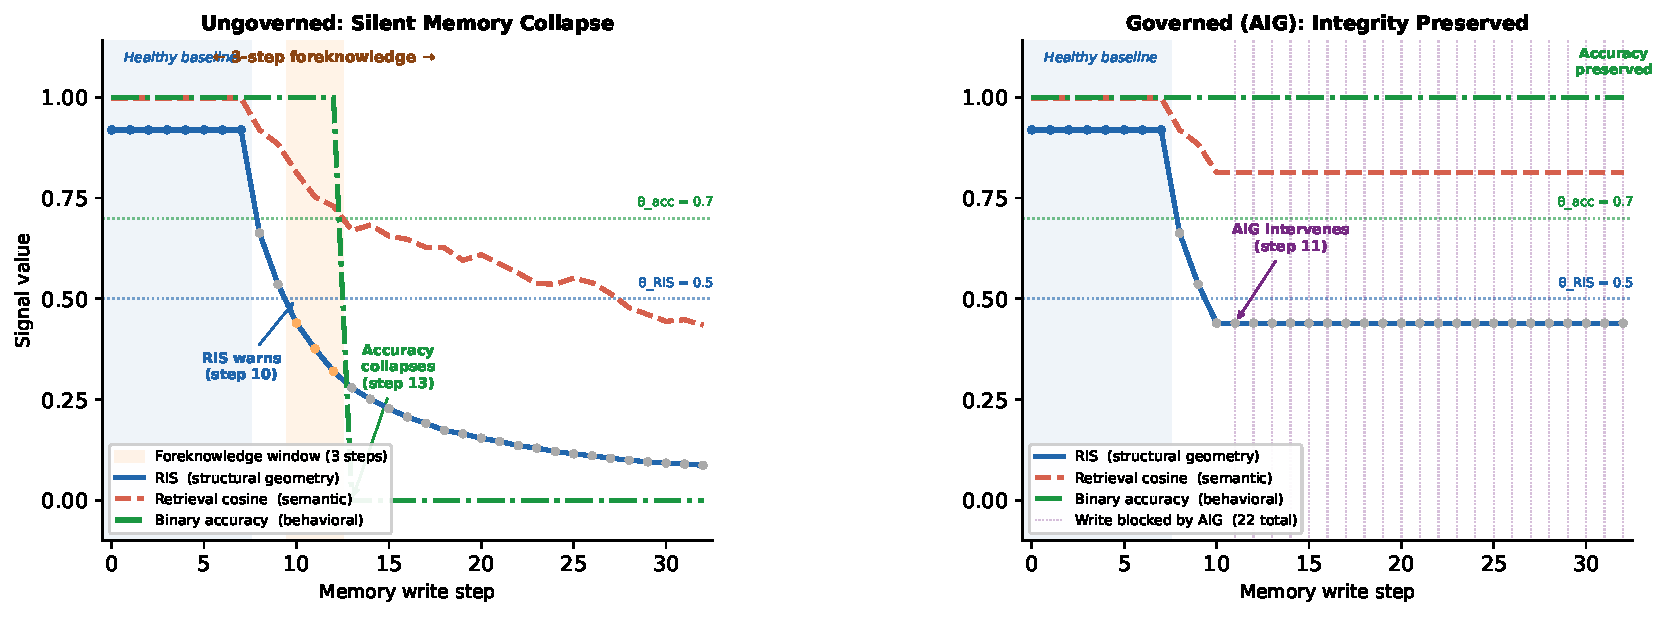
\includegraphics[width=\linewidth]{fig_hidden_collapse}
\caption{\textbf{Hidden Memory Collapse: structural failure precedes behavioral
failure---RIS detects imminent degradation before retrieval quality or accuracy
deteriorates.}
($d{=}128$, interferer $\cos{\approx}0.42$, 25 writes attempted.)
\emph{Left:} 3-step \emph{foreknowledge window} between RIS warning (step~10)
and accuracy cliff (step~13)---memory geometrically failing while outputs appear
correct.
\emph{Right:} AIG blocks 22 of 25 writes; accuracy preserved at 1.0 throughout.
Ungov.\ final: RIS$\,{=}\,0.087$, acc$\,{=}\,0.0$.
Gov.\ final: RIS$\,{=}\,0.440$, acc$\,{=}\,1.0$.}
\label{fig:hidden_collapse}
\end{figure*}

\paragraph{Stability lead-time (E8).}
Across $d{\in}\{64,128,256\}$, interferer cosine ${\approx}\{0.25,0.42,0.58\}$,
$N{=}30$ trials per condition (270 total, $\tau{=}0.75$):
RIS precedes behavioral failure in \textbf{94.4\%} of trials
(255/270; 95\% CI: 91--97\%), mean lead $3.15{\pm}2.78$ steps---from
${\sim}6.7$ steps at low cosine (100\%) to ${\sim}0.84$ at high cosine
(${\approx}83\%$, where interferer keys approach the anchor's geometry).
The decay $\Delta \propto \mu_{\cos}^{-2.16}$ ($R^2{=}0.979$) makes the window
predictable; the 3.15-step lead ($\tau{=}0.75$, all regimes) and the 15.9-step
lead (quality${<}0.50$, mid-range, \S\ref{sec:memo_governance}) measure the
same precursor under different operational thresholds.
Operationally, 3 steps is sufficient: P2 rollback or $\alpha$ reduction
executes in $O(d^2)$, within a single memory-update cycle.
\emph{Threshold robustness:} positive rate is identical at
$\theta_{\mathrm{RIS}}{\in}\{0.65,0.75\}$ (94.4\% at both values); at
$\theta{=}0.55$ it falls to 59.3\%, confirming the result is stable across
the upper-threshold regime and not a single-choice artifact.

\paragraph{Semantic validation across model families.}
To confirm the foreknowledge window is not a random-geometry artifact,
we test 3 sentence-embedding model families across 4 domains
(60 contamination writes per trial, 6 anchor rotations per domain;
$\theta_{\mathrm{RIS}}{=}0.50$, below E8's operational $\theta{=}0.65$;
Table~\ref{tab:semantic}).
Across all 49 evaluated trials, the foreknowledge window is \textbf{100\%
positive}---structural warning precedes behavioral failure in every case.
Mean $\Delta{=}26.5{\pm}2.7$ steps at $\mu_{\cos}{\approx}0.26$--$0.28$
(low semantic cosine regime): consistent with the decay law, which predicts
larger windows at lower cosine concentration.
These results suggest the effect is a property of explicit associative memory
architecture rather than an artifact of controlled random geometry.

\begin{table}[h]
\centering
\caption{\textbf{Foreknowledge window across sentence-embedding families.}
3 models $\times$ 4 domains, 60 contamination writes/trial;
$\theta_{\RIS}{=}0.50$, $\theta_{\mathrm{acc}}{=}0.70$.}
\label{tab:semantic}
\vspace{-2pt}
\small
\begin{tabular}{@{}lcccc@{}}
\toprule
Model & $d$ & $\mu_{\cos}$ & $\Delta$ (steps) & Pos.\,\% \\
\midrule
all-MiniLM-L6-v2      & 384 & 0.264 & $27.2{\pm}6.7$  & 100\% \\
all-mpnet-base-v2     & 768 & 0.280 & $29.3{\pm}10.8$ & 100\% \\
paraphrase-MiniLM-L6  & 384 & 0.270 & $22.9{\pm}5.3$  & 100\% \\
\midrule
\textbf{Overall}      &     & 0.271 & $\mathbf{26.5{\pm}2.7}$ & \textbf{100\%} \\
\bottomrule
\end{tabular}
\end{table}

\paragraph{Governance and failure mode validation.}
F1/F2 write-gate: 0.552$\to$0.813 accuracy.
F3 (permutation aliasing, silent to RIS): circular-convolution keys recover 50\%$\to$100\%, a known scope boundary.
F4: RIS-quality correlation $\rho{=}0.938{\pm}0.019$.
F6 budget $B_{\max}$: 97\% adversarial block rate ($\cos{=}0.45$, $N{=}60$; quality 0.31$\to$0.807).
40\% RIS false-negative rate confined to dominant-wrong-key injection;
0/500 within-domain (95\% CI: 0--0.7\%; explicit FN tracking).

% ---------------------------------------------------------------
\section{Extending MeMo: From Explicit Storage to Operational Accountability}
\label{sec:memo_governance}

MeMo's explicit outer-product architecture makes stored associations directly
inspectable~\citep{zanzotto2025memo}; this work shows it also makes operations
\emph{accountable}---write consequences computable before execution rather than
discovered after.
At MeMo's production scale ($d{=}2048$, chunk length 384), P3 confirms that
MeMo's chunk-length design keeps each CMM inside the RIS-stable capacity region.

\textbf{Three capabilities MeMo's structure unlocks}
(GovernedMeMoLayer, a drop-in replacement for MeMo's \texttt{MeMoLayer}):
\emph{Exact removal} (P2): each outer-product association is removed algebraically
exactly---to within $3{\times}10^{-8}$ in float32---filling a gap in MeMo's existing
\texttt{forget()} interface.
\emph{Pre-execution interference} (P1): any write's perturbation is computable
in $O(P)$ before execution, algebraically unavailable in parametric models.
\emph{Continuous health} (RIS-$\alpha$): a RIS-adaptive $\alpha$ replaces fixed
$\alpha{=}0.5$ with retrieval trust derived from live geometric state.
The 40.7\% block rate applies under adversarial injection.

\textbf{Experimental validation} ($N{=}30$ trials, $d{=}128$,
interferer cosine ${\in}[0.25,0.58]$; Figure~\ref{fig:memo_governance}).
\emph{(A) Predictive failure:} RIS drops below $\theta{=}0.65$ an average
of $\mathbf{15.9{\pm}6.7}$ steps before quality drops below 0.50 in
\textbf{100\%} of trials---failure is structurally visible before it is
behaviorally observable.
\emph{(B) Intervention efficacy:} without governance, quality degrades to
$0.235{\pm}0.087$; P1 gating and P2 rollback recover it to
$\mathbf{0.957{\pm}0.002}$ ($\mathbf{+0.722}$).
\emph{(C) Adaptive alpha:} RIS-adaptive $\alpha$ outperforms MeMo's fixed
$\alpha{=}0.5$ by $+109.2\%$ at $P{=}100$ (transformer baseline quality 0.85).

\begin{figure}[t]
\centering
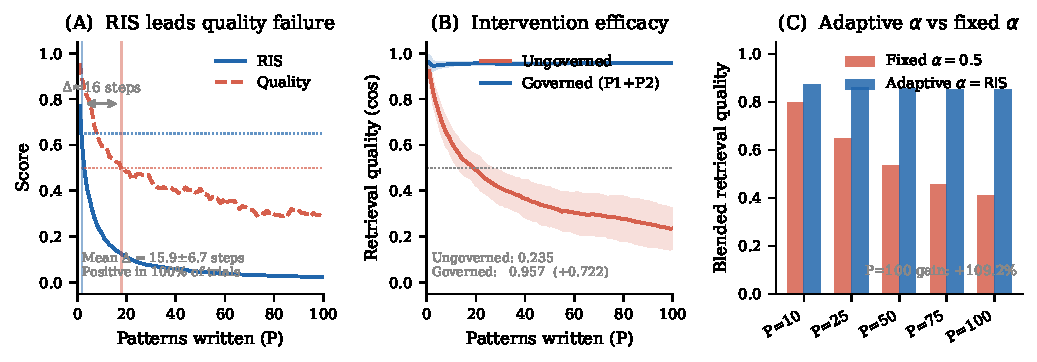
\includegraphics[width=\linewidth]{fig_memo_governance}
\caption{\textbf{Operational capabilities of explicit associative memory,
applied to a MeMo-style CMM layer} ($d{=}128$, $N{=}30$ trials).
\textbf{(A)} RIS exposes latent degradation $15.9{\pm}6.7$ steps before quality
failure (100\% of trials).
\textbf{(B)} P1+P2 provide exact interference bounds and exact rollback:
quality recovers from $0.235$ to $0.957$ ($+0.722$).
\textbf{(C)} RIS-adaptive $\alpha$ provides continuous health monitoring: $+109.2\%$
in retrieval quality over fixed $\alpha{=}0.5$ at $P{=}100$.}
\label{fig:memo_governance}
\end{figure}

% ---------------------------------------------------------------
\section{Scope, Limitations, and PhD Research Plan}
\label{sec:open}

All results hold within single-layer CMM scope; P1 is exact in any geometric
regime; P3 requires per-embedding recalibration for semantic keys.
Four honest limitations:

\begin{table}[h]
\centering
\caption{\textbf{Scope and limitations.}}
\label{tab:limitations}
\small
\begin{tabular}{@{}p{2.0cm}p{4.8cm}@{}}
\toprule
\textbf{Limitation} & \textbf{Description} \\
\midrule
RIS false negatives
  & $40\%$ under dominant-wrong-key injection; 0/500 within-domain
    (95\% CI: 0--0.7\%) \\[3pt]
Multi-layer scope
  & P2 exact per layer; ghost keys persist in derived layers (F5, below) \\[3pt]
P3 regime
  & Random geometry; semantic embeddings require per-embedding recalibration
    ($7$--$9{\times}$ measured for BERT) \\[3pt]
CMM substrate
  & FFN layers are key-value memories~\citep{geva2021transformer};
    certificate extension requires non-linear theory (Year~2+ scope) \\
\bottomrule
\end{tabular}
\end{table}

\textbf{F5: The central open problem and PhD thesis target.}
Single-layer certificates do not compose across MeMo layers
(Figure~\ref{fig:multilayer}): removing a pattern from layer $\ell$ leaves its
derived key $f(s_1) = s_1^\top\mathbf{C}_1$ in layer $\ell{+}1$ as a ghost
from a prior CMM state---confirmed in MeMo's production \texttt{forget()}
interface, where intermediate layers accumulate rather than subtract associations.
Adversarial experiments show $\varepsilon_{L_2}/\varepsilon_{L_1}$ reaching
$1.98\times$ (mean $1.07\times$)---interference amplifies across layers, so
certificates computed for L1 underestimate downstream perturbation.
F5 is not a peripheral limitation but the mathematical condition under which
AIG cannot yet guarantee full accountability across MeMo's stacked layers;
resolving it is the Year~1 thesis target.

\begin{figure}[t]
\centering
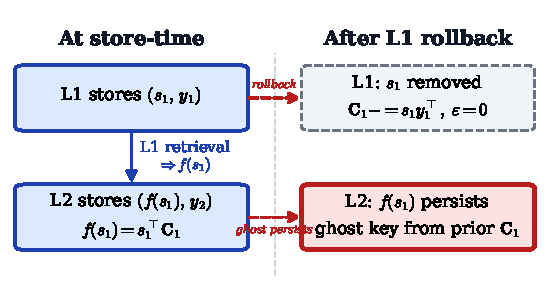
\includegraphics[width=\linewidth]{fig_multilayer_rollback}
\caption{\textbf{Multi-layer rollback limitation (F5).} P2 is exact per layer.
$f(s_1){=}s_1^\top\mathbf{C}_1$ is computed at store-time; after L1 rollback
$\mathbf{C}_1$ is gone but $f(s_1)$ persists in L2 as a ghost key.
Joint certificate composition across state-derived layers is the open problem.}
\label{fig:multilayer}
\end{figure}

\textbf{PhD research plan} (three phases, within the MeMo project):
(1)~\emph{Year~1}---solve F5: derive a joint interference certificate for stacked
CMMs and validate P2 exact rollback at MeMo's full production scale;
(2)~\emph{Year~2}---test ACS (Attentional Coherence Score): the hypothesis is
that a RIS-analogous concentration statistic on transformer attention weights
predicts factual-recall failure before behavioral collapse on held-out QA
benchmarks, via a Modern Hopfield Network bridge~\citep{ramsauer2021hopfield};
(3)~\emph{Year~3}---deliver a unified governance framework with formal
accountability across CMMs, Hopfield networks, and attention, as deployment-ready
extensions to MeMo's full language-model stack.

\textbf{Contribution attribution.}
MeMo architecture, forgetting interface, and \texttt{directly\_forget()} are due
to Zanzotto et al.~\citep{zanzotto2025memo}; AIG instruments MeMo's substrate
rather than modifying it. Theory, taxonomy, experiments, and F5 discovery are the PhD
author's contribution, developed as an extension of MeMo's accountability theory.

% ---------------------------------------------------------------
\begin{acknowledgments}
The author thanks Prof.\ Fabio Massimo Zanzotto (University of Rome Tor Vergata)
for supervision and for the foundational MeMo architecture on which this work
is built.
\end{acknowledgments}

% ---------------------------------------------------------------
\begin{thebibliography}{99}

\bibitem[Cabannes et al., 2024]{cabannes2024scaling}
Cabannes, V., Dohmatob, E., and Bietti, A. (2024).
\newblock Scaling laws for associative memories.
\newblock In \emph{Proceedings of the International Conference on Learning
  Representations (ICLR 2024)}.

\bibitem[Geva et al., 2021]{geva2021transformer}
Geva, M., Schuster, R., Berant, J., and Levy, O. (2021).
\newblock Transformer feed-forward layers are key-value memories.
\newblock In \emph{Proceedings of EMNLP 2021}, pages 9484--9495.

\bibitem[Guo et al., 2020]{guo2020certified}
Guo, C., Goldstein, T., Hannun, A., and van~der Maaten, L. (2020).
\newblock Certified data removal from machine learning models.
\newblock In \emph{Proceedings of ICML 2020}, pages 3832--3842.

\bibitem[Kirkpatrick et al., 2017]{kirkpatrick2017overcoming}
Kirkpatrick, J., Pascanu, R., Rabinowitz, N., Veness, J., Desjardins, G.,
  Rusu, A.~A., Milan, K., Quan, J., Ramalho, T., Grabska-Barwinska, A.,
  Hassabis, D., Clopath, C., Kumaran, D., and Hadsell, R. (2017).
\newblock Overcoming catastrophic forgetting in neural networks.
\newblock \emph{Proceedings of the National Academy of Sciences},
  114(13):3521--3526.

\bibitem[Kohonen, 1972]{kohonen1972correlation}
Kohonen, T. (1972).
\newblock Correlation matrix memories.
\newblock \emph{IEEE Transactions on Computers}, 21(4):353--359.

\bibitem[L{\'o}pez-Paz and Ranzato, 2017]{lopez2017gradient}
L{\'o}pez-Paz, D. and Ranzato, M. (2017).
\newblock Gradient episodic memory for continual learning.
\newblock In \emph{Advances in Neural Information Processing Systems
  (NeurIPS 2017)}.

\bibitem[Ramsauer et al., 2021]{ramsauer2021hopfield}
Ramsauer, H., Sch\"{a}fl, B., Lehner, J., Seidl, P., Widrich, M.,
  Adler, T., Gruber, L., Holzleitner, M., Pavlovi\'{c}, M.,
  Sandve, G.~K., Greiff, V., Kreil, D., Kopp, M., Klambauer, G.,
  Brandstetter, J., and Hochreiter, S. (2021).
\newblock {Hopfield} networks is all you need.
\newblock In \emph{Proceedings of ICLR 2021}.

\bibitem[Zanzotto et al., 2025]{zanzotto2025memo}
Zanzotto, F.~M. et al. (2025).
\newblock {MeMo}: Towards language models with associative memory mechanisms.
\newblock In \emph{Findings of ACL 2025}, pages 15169--15180, Vienna, Austria.

\end{thebibliography}

\end{document}
